%%%%%%%%%%%%%%%%%%%%%%%%%%%%%%%%%%%%%%%%%
% baposter Landscape Poster
% LaTeX Template
% Version 1.0 (11/06/13)
%
% baposter Class Created by:
% Brian Amberg (baposter@brian-amberg.de)
%
% This template has been downloaded from:
% http://www.LaTeXTemplates.com
%
% License:
% CC BY-NC-SA 3.0 (http://creativecommons.org/licenses/by-nc-sa/3.0/)
%
%%%%%%%%%%%%%%%%%%%%%%%%%%%%%%%%%%%%%%%%%

%----------------------------------------------------------------------------------------
%	PACKAGES AND OTHER DOCUMENT CONFIGURATIONS
%----------------------------------------------------------------------------------------

\documentclass[landscape,a0paper,fontscale=0.285]{baposter} % Adjust the font scale/size here

\usepackage{graphicx} % Required for including images
\graphicspath{{figures/}} % Directory in which figures are stored

\usepackage{amsmath} % For typesetting math
\usepackage{amssymb} % Adds new symbols to be used in math mode

\usepackage{booktabs} % Top and bottom rules for tables
\usepackage{enumitem} % Used to reduce itemize/enumerate spacing
\usepackage{palatino} % Use the Palatino font
\usepackage[font=small,labelfont=bf]{caption} % Required for specifying captions to tables and figures

\usepackage{multicol} % Required for multiple columns
\setlength{\columnsep}{1.5em} % Slightly increase the space between columns
\setlength{\columnseprule}{0mm} % No horizontal rule between columns

\usepackage{tikz} % Required for flow chart
\usetikzlibrary{shapes,arrows} % Tikz libraries required for the flow chart in the template

\newcommand{\compresslist}{ % Define a command to reduce spacing within itemize/enumerate environments, this is used right after \begin{itemize} or \begin{enumerate}
\setlength{\itemsep}{1pt}
\setlength{\parskip}{0pt}
\setlength{\parsep}{0pt}
}

\definecolor{lightblue}{rgb}{0.145,0.6666,0.9} % Defines the color used for content box headers
\definecolor{black}{rgb}{0.2,0.2,0.2}
\begin{document}

\begin{poster}
{
headerborder=closed, % Adds a border around the header of content boxes
colspacing=0.7em, % Column spacing
bgColorOne=white, % Background color for the gradient on the left side of the poster
bgColorTwo=white, % Background color for the gradient on the right side of the poster
borderColor=lightblue, % Border color
headerColorOne=black, % Background color for the header in the content boxes (left side)
headerColorTwo=lightblue, % Background color for the header in the content boxes (right side)
headerFontColor=white, % Text color for the header text in the content boxes
boxColorOne=white, % Background color of the content boxes
textborder=roundedleft, % Format of the border around content boxes, can be: none, bars, coils, triangles, rectangle, rounded, roundedsmall, roundedright or faded
eyecatcher=true, % Set to false for ignoring the left logo in the title and move the title left
headerheight=0.1\textheight, % Height of the header
headershape=roundedright, % Specify the rounded corner in the content box headers, can be: rectangle, small-rounded, roundedright, roundedleft or rounded
headerfont=\Large\bf\textsc, % Large, bold and sans serif font in the headers of content boxes
%textfont={\setlength{\parindent}{1.5em}}, % Uncomment for paragraph indentation
linewidth=1.5pt % Width of the border lines around content boxes
}
%----------------------------------------------------------------------------------------
%	TITLE SECTION 
%----------------------------------------------------------------------------------------
%
{
\includegraphics[height=8em]{wits.jpg}} % First university/lab logo on the left
{\bf\textsc{An investigational study into the design of a low cost, adaptive hearing aid}\vspace{0.3em}} % Poster title
{\textsc{ Kayla-Jade Butkow \& Kelvin da Silva \hspace{12pt} {\small School of Electrical \& Information Engineering, University of the Witwatersrand}}} % Author names and institution
{
\includegraphics[height=8em]{EIE.pdf}} % Second university/lab logo on the right

%----------------------------------------------------------------------------------------
%	INTRODUCTION
%----------------------------------------------------------------------------------------

\headerbox{Introduction}{name=introduction,column=0,row=0}{

Hearing loss is a prevalent problem that affects people in all parts of the world. It is caused by many factors including age, disease and trauma, and often results in a decreased quality of life for people suffering from it \cite{Evaluation_of_a_hearing_compensation_algorithm}. Hearing aids that exist on the market are expensive, and are thus inaccessible to the majority of the population, particularly in South Africa. It is therefore necessary to develop an inexpensive hearing aid that has all of the functionality of a high-end hearing aid.

This functionality includes:
\begin{itemize}\compresslist
	\item The application of specific amplifications to specific frequency bands according to a person's audiogram
	\item The ability of the user to select the direction in which they wish to listen and to hear that direction louder than other directions
\end{itemize}
}

%----------------------------------------------------------------------------------------
%	OBJECTIVES
%----------------------------------------------------------------------------------------

\headerbox{Objectives}{name=objectives,column=0,below=introduction}{
	\begin{itemize}\compresslist
		\item To create a full software simulation of a hearing aid
		\item To create a hardware proof of concept of a hearing aid which demonstrates limited functionality
	\end{itemize}
}

%----------------------------------------------------------------------------------------
%	FUTURE WORK
%----------------------------------------------------------------------------------------

\headerbox{Future Work}{name=FutureWork,column=3,row=0,bottomaligned=introduction}{
This project has been a proof of concept that an inexpensive adaptive hearing aid can be produced. For future development of the hearing aid, a number of improvements could be made including:
\begin{itemize}\compresslist
	\item Making use of higher quality omni-directional microphones
	\item Creating an integrated circuit chip to handle the preprocessing of the audio signals
	\item Making use of more microphones to improve the precision of the directionality feature
\end{itemize}
}


%----------------------------------------------------------------------------------------
%	METHODOLOGY
%----------------------------------------------------------------------------------------

\headerbox{Methodology}{name=method,column=0,below=objectives, above=bottom}{ % This block's bottom aligns with the bottom of the conclusion block

{\Large \textbf{Simulated Hearing Aid}}\\
block diagram

{\Large \textbf{Hardware Hearing Aid}}\\
block diagram

{\Large \textbf{Testing}}
\begin{itemize}\compresslist
	\item Hearing aid placed on a rotating platform and rotated in ${30}^o$ increments with a constant direction selected on the device
	\item Sinusoidal signals with frequencies of 3340~Hz and 6000~Hz were played from a set direction and the output signals from the hearing aid were recorded
	\item Different amplifications were applied to the two frequency bands and the input and output signals were recorded
\end{itemize}

\begin{center}
	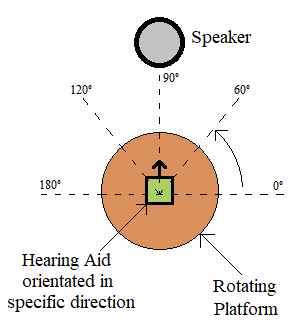
\includegraphics[width=0.8\linewidth]{directionalityLabTest.png}
	\captionof{figure}{Procedure for testing the hearing aid}
\end{center}

}


%----------------------------------------------------------------------------------------
%	CONCLUSION
%----------------------------------------------------------------------------------------

\headerbox{Conclusion}{name=conclusion,column=3,below=FutureWork}{ % This block's bottom aligns with the bottom of the conclusion block
	
}

%----------------------------------------------------------------------------------------
%	REFERENCES
%----------------------------------------------------------------------------------------

\headerbox{References}{name=references,column=3,above=bottom, below=conclusion}{
	
	\renewcommand{\section}[2]{\vskip 0.05em} % Get rid of the default "References" section title
	\nocite{*} % Insert publications even if they are not cited in the poster
	\small{ % Reduce the font size in this block
		\bibliographystyle{unsrt}
		\bibliography{sample} % Use sample.bib as the bibliography file
}}

%----------------------------------------------------------------------------------------
%	RESULTS
%----------------------------------------------------------------------------------------

\headerbox{Results}{name=results,column=1,span=2,row=0, bottomaligned=references}{

\begin{multicols}{2}
\vspace{1em}

\end{multicols}

%------------------------------------------------

\begin{multicols}{2}
\vspace{1em}


\end{multicols}
}


%----------------------------------------------------------------------------------------

\end{poster}

\end{document}